% Figure 3: the real reference pre-training run (BPE_REPORT curve, verbatim)
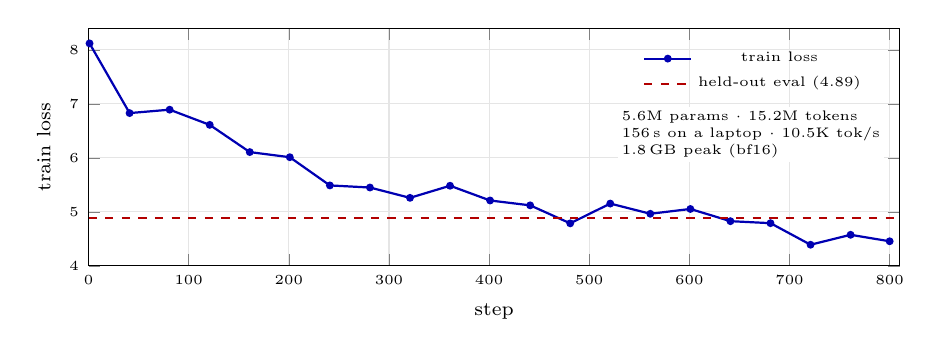
\begin{tikzpicture}
\begin{axis}[
  width=0.98\columnwidth, height=4.6cm,
  xlabel={step}, ylabel={train loss},
  xmin=0, xmax=810, ymin=4, ymax=8.4,
  tick label style={font=\tiny}, label style={font=\scriptsize},
  legend style={font=\tiny, draw=none, fill=none, at={(0.97,0.95)}, anchor=north east},
  grid=major, grid style={gray!20},
]
\addplot[color=blue!70!black, thick, mark=*, mark size=1pt]
  coordinates {(1,8.119)(41,6.829)(81,6.892)(121,6.611)(161,6.107)(201,6.012)
               (241,5.490)(281,5.451)(321,5.260)(361,5.484)(401,5.211)(441,5.121)
               (481,4.788)(521,5.154)(561,4.965)(601,5.054)(641,4.828)(681,4.791)
               (721,4.392)(761,4.576)(800,4.456)};
\addlegendentry{train loss}
\addplot[color=red!70!black, dashed, thick] coordinates {(0,4.886)(810,4.886)};
\addlegendentry{held-out eval (4.89)}
\node[font=\tiny, align=left, anchor=north east, fill=white, inner sep=1.5pt]
  at (axis cs:795,6.95)
  {5.6M params $\cdot$ 15.2M tokens\\ 156\,s on a laptop $\cdot$ 10.5K tok/s\\ 1.8\,GB peak (bf16)};
\end{axis}
\end{tikzpicture}
